\begin{figure}[p]
\centering
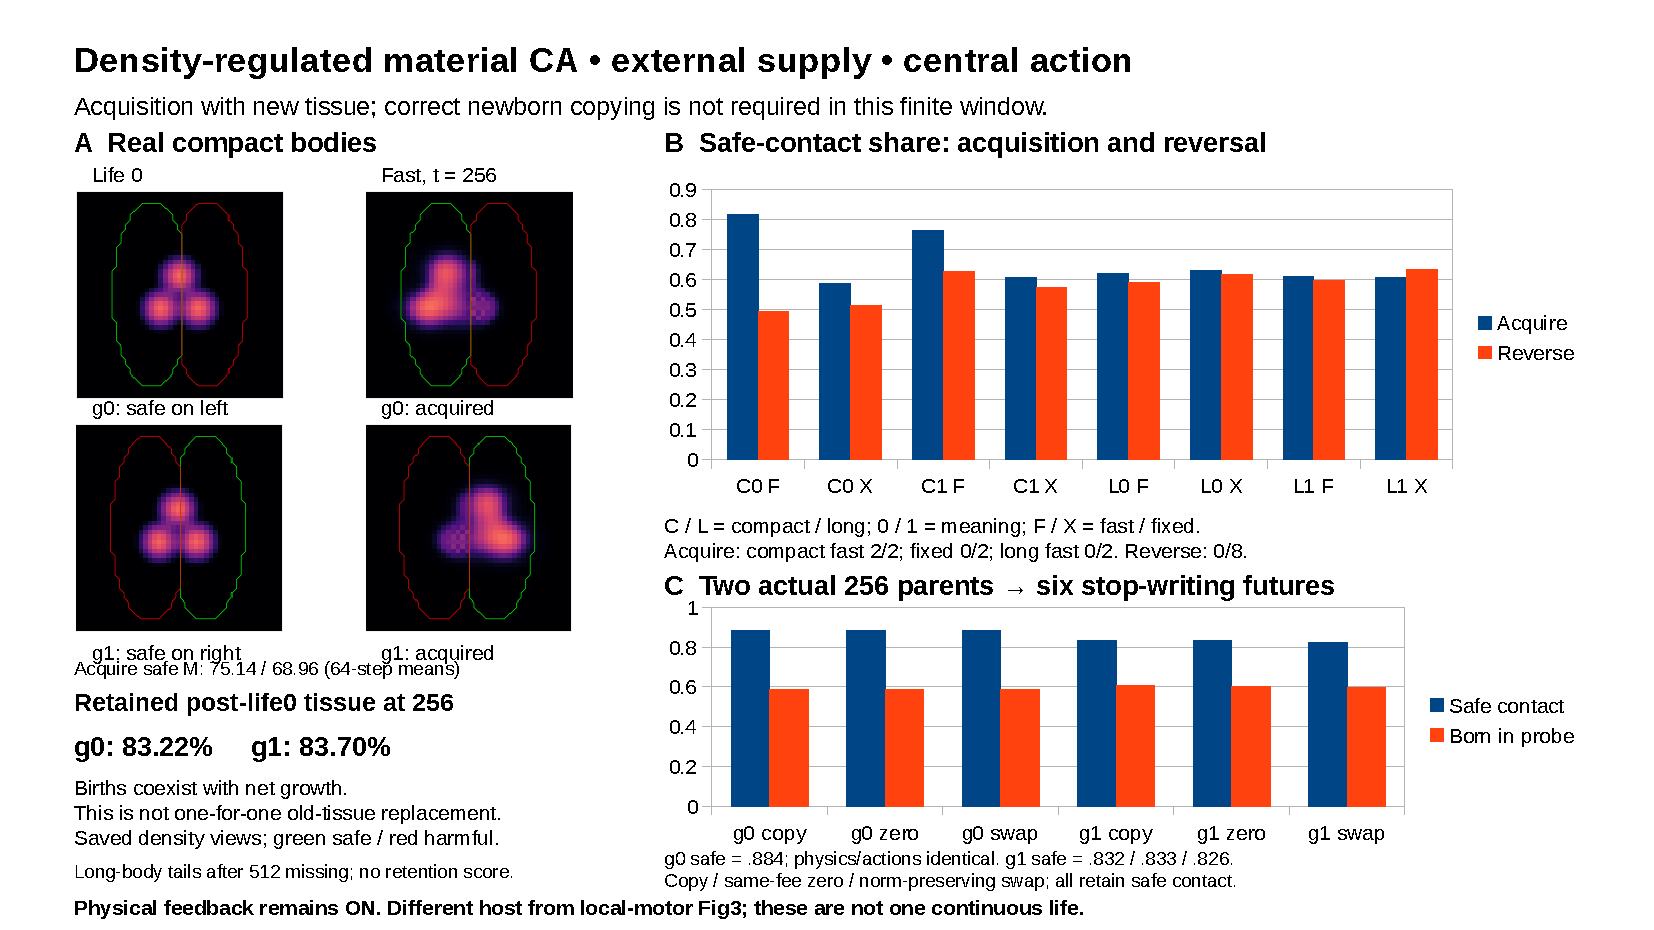
\includegraphics[width=\linewidth,height=0.72\textheight,keepaspectratio]{work/longform_v047/figures/young_turnover_v0475/young_turnover.pdf}
\captionsetup{font=footnotesize}
\caption{\textbf{Conditional acquisition during real tissue production in a distinct host.}
\textbf{a}, Actual compact density fields at life zero and acquired step 256. Green/red contours mark safe/harmful regions; these are density views, not spatial birth-cohort maps. Post-life-zero tissue constitutes $83.22\%$ and $83.70\%$ of the two acquired bodies. Births accompany net growth, so these shares do not measure one-for-one founder replacement.
\textbf{b}, Final-64 safe-contact fractions for all eight geometry--meaning--controller conditions. Compact fast acquisition passes $2/2$, compact fixed prior $0/2$, elongated fast $0/2$; all eight fail complete reversal. Success also requires absolute contact, viability and tissue criteria. The elongated expression tails after 512 are missing.
\textbf{c}, Two actual acquired parents each provide copy, same-tariff zero and norm-preserving swap futures. Writing stops for 128 steps, while physical energetic feedback continues. Safe contact is a final-64 mean; born-in-probe bars are endpoint retained fractions. All six related futures pass; the first parent's physical/action histories coincide. Correct newborn copying is therefore unnecessary in this tested window, with surviving old contents intact. This externally supplied density-regulated material CA has central action and differs from both original Lenia generation and the no-birth scalar-action host in Fig.~\ref{fig:scalar-action}.}
\label{fig:young-turnover}
\end{figure}
